\chapter{Distribucion de Radiofrecuencias en Argentina}
El Espectro Radioeléctrico es el conjunto de frecuencias que, conforme a la tecnología disponible, 
pueden ser empleadas para emitir ondas que permitan transportar información como voz, datos, 
imágenes, sonidos, etc.

Una de las principales características es que se trata de un medio finito. Es decir que una vez 
ocupada una frecuencia específica por una persona, ésta no puede ser utilizada por otra y existen 
una cantidad limitada de bandas de frecuencias que pueden ser empleadas.

\begin{figure}[ht]
    \begin{center}
        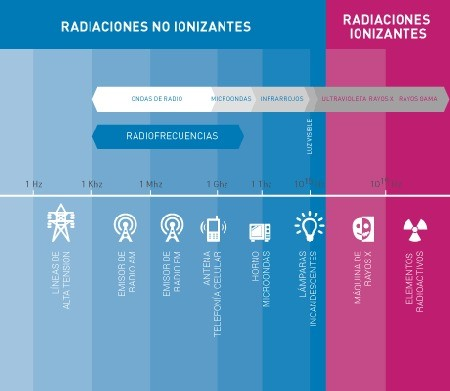
\includegraphics{contenido/img/radiofrecuencias.jpg}
        \caption{Radiofrecuencias en Argentina}
        \label{fig:rad_frec}
    \end{center}
\end{figure}

La siguiente tabla muestra las frecuencias de operación y los niveles de potencia que emiten los 
diversos Servicios y Sistemas de Comunicaciones Radioeléctricas:
\begin{table}[ht]
    \begin{center}
        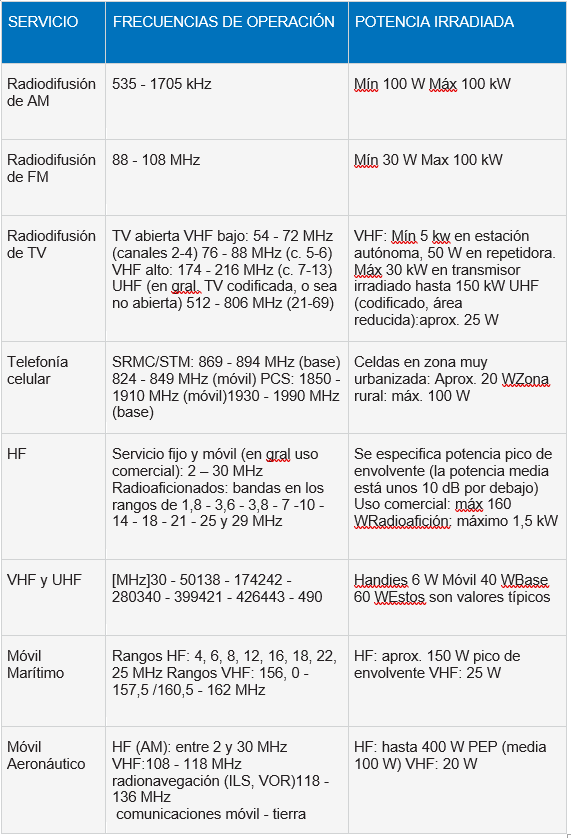
\includegraphics{contenido/img/tablaej5.png}
    \end{center}
\end{table}

